\RequirePackage{silence} % :-\
  \WarningFilter{scrreprt}{Usage of package `titlesec'}
  \WarningFilter{titlesec}{Non standard sectioning command}
\documentclass[11pt,
  footinclude,headinclude,
  abstract=on
]{scrreprt}
%paper=b5

%% %%%%%%%%%%%%%%%%%%%%%%%%%%%%%%%%%%%%%%%%%%%%%%%%%%%%%%%%%%%%%%%%%%%%%%
%% ************************************************************
%% ==================================================

%% General
%% %%%%%%%%%%%%%%%%%%%%%%%%%%%%%%%%%%%%%%%%%%%%%%%%%%%%%%%%%%%%%%%%%%%%%%

\usepackage[T1]{fontenc}
\usepackage[linedheaders=true]{classicthesis} % ,manychapters
%\usepackage[osf]{libertine}
\usepackage[english]{babel}

%% Bibliography
%% %%%%%%%%%%%%%%%%%%%%%%%%%%%%%%%%%%%%%%%%%%%%%%%%%%%%%%%%%%%%%%%%%%%%%%

\usepackage{natbib}
%% Settings copied from the ACM style
\bibliographystyle{ACM-Reference-Format}{}
\setcitestyle{%
    authoryear,%
    open={[},close={]},citesep={;},%
    aysep={},yysep={,},%
    notesep={, }}
\let\citeN\cite
\let\cite\citep

%% Style
%% %%%%%%%%%%%%%%%%%%%%%%%%%%%%%%%%%%%%%%%%%%%%%%%%%%%%%%%%%%%%%%%%%%%%%%

\usepackage{xspace}
\usepackage{xcolor}

%% Math
%% %%%%%%%%%%%%%%%%%%%%%%%%%%%%%%%%%%%%%%%%%%%%%%%%%%%%%%%%%%%%%%%%%%%%%%



\begin{document}

%% General
%% ======================================================================

\newcommand{\TODO}[1]{\textcolor{red}{\textbf{TODO:} #1}}

\newcommand{\figref}[1]{Fig.~\ref{#1}\xspace}
\newcommand{\lemref}[1]{Lem.~\ref{#1}\xspace}
\newcommand{\thmref}[1]{Thm.~\ref{#1}\xspace}
\newcommand{\ruleref}[1]{Rule~{\small #1}\xspace}
\newcommand{\defref}[1]{Def.~\ref{#1}\xspace}
\newcommand{\secref}[1]{Section~\ref{#1}\xspace}
\newcommand{\chapref}[1]{Chapter~\ref{#1}\xspace}
\newcommand{\appref}[1]{Appendix~\ref{#1}\xspace}

\newcommand{\tdef}[1]{\textbf{#1}}

\newcommand{\CSharp}{C\texttt{\small\#}\xspace}
\newcommand{\FSub}{$F^N_{\leq}$\xspace}

%% for wide figures:
%% http://16marzo.blogspot.com/2009/09/figure-e-margini-in-classicthesis.html
\newlength\largefigure
\setlength{\largefigure}{\columnwidth+\marginparsep+\marginparwidth}

\definecolor{light-gray}{gray}{0.85}

\newcommand{\cfbox}[2]{%
    \colorlet{currentcolor}{.}%
    {\color{#1}%
    \fbox{\color{currentcolor}#2}}%
}

%% Code
%% *********************************************************

\newcommand{\code}[1]{\texttt{\small#1}\xspace}
\newcommand{\cjl}[1]{\lstinline[language=Julia]!#1!\xspace}

\lstnewenvironment{julia}
    {\lstset{language=Julia,numbers=left,}}
    {}
\newenvironment{codeenvd}
    {
    \begin{center}
    \begin{minipage}{8cm}
    }
    {
    \end{minipage}
    \end{center}
    }

%% Math
%% *********************************************************

%% make sure we are in math mode
\newcommand{\EM}[1]{\ensuremath{#1}\xspace}

\newtheorem{theorem}{Theorem}
\newtheorem{lemma}{Lemma}

\newcommand{\interp}[1]{\EM{\llbracket #1 \rrbracket}}

%% Formalization
%% ======================================================================

%% Metavariables
%% *********************************************************

\newcommand{\ty}{\EM{\tau}}                 %% type annotation τ
\newcommand{\gty}{\EM{\sigma}}              %% type tag σ

\newcommand{\nsty}{\EM{\phi}}               %% normalized simple type φ
%% normalized existential type
\newcommand{\nety}{\EM{\xi}}
%\newcommand{\nety}{\EM{\prescript{\exists}{}{\phi}}}        %% ∃φ
%% normalized union-existential type
\newcommand{\nuty}{\EM{\omega}}
%\newcommand{\nuty}{\EM{\prescript{}{\cup\exists}{\phi}}}    %% ∪∃φ       


\newcommand{\cname}{\EM{\mathit{cname}}}
\newcommand{\aname}{\EM{\mathit{aname}}}
\newcommand{\iname}{\EM{\mathit{name}}}

\newcommand{\VEnv}{\EM{\mathrm{V}}}     %% simple variable environment V
\newcommand{\AEnv}{\EM{\Gamma}}         %% forall-variable environment Γ
\newcommand{\EEnv}{\EM{\mathbf\Delta}}         %% exist-variable environment Δ
                                        %% (unification variables)
\newcommand{\EmptyEnv}{\EM{\cdot}}

\newcommand{\CSet}{\EM{\mathcal{C}}}    %% set of subtype constraints
\newcommand{\EmptySet}{\EM{\varnothing}}    %% empty set of constraints

%% Style
%% *********************************************************

\newcommand{\tyname}[1]{\EM{\mathsf{#1}}}       %% type name (like Int)
\newcommand{\var}[1]{\EM{\mathrm{#1}}}          %% type variable
\newcommand{\unvar}[1]{\EM{\mathbf{#1}}}        %% unification variable

%% overline for list
\newcommand{\ol}[1]{\EM{\overline{#1}}}

%% set
\newcommand{\cset}[1]{\EM{\{#1\}}}

%% side condition
\newcommand{\sidecond}[1]{\EM{\scriptstyle #1}}

%% inference rule names
\newcommand{\SR}[1]{\textsc{S-#1}}
\newcommand{\ER}[1]{\textsc{E-#1}}

%% Symbols
%% *********************************************************

\newcommand{\Alt}{~\vert~}                      %% |

\newcommand{\symsub}{\EM{<:}}                   %% <:
\newcommand{\symeq}{\EM{\approx}}               %% ==
%\newcommand{\vdashfr}{\EM{\vdash\!\!{\circ}}}   %% |-o
\newcommand{\vdashfr}{\EM{\Vdash}}   %% ||-

%% Type Constructors
%% *********************************************************

\newcommand{\tyany}{\tyname{Any}}               %% Any
\newcommand{\tybot}{\tyname{Bot}}               %% Bot

\newcommand{\typair}[2]{\EM{#1 \times #2}}      %% t1 × t2
\newcommand{\tyunion}[2]{\EM{#1 \cup #2}}       %% t1 ∪ t2

\newcommand{\tyinv}[2]{\EM{#1\{#2\}}}           %% t1{...}

%\newcommand{\tybound}[3]{\EM{\tyvar{#1}\!\in\!({#2},{#3})}} %% X \in (tl,tu)
\newcommand{\varbound}[3]{\EM{#2\!\symsub\!#1\!\symsub\!#3}} %% tl<:X<:tu
\newcommand{\tybound}[3]{\varbound{\tyvar{#1}}{#2}{#3}} %% tl<:X<:tu
\newcommand{\tyboundu}[2]{\EM{\tyvar{#1}\!\symsub\!#2}}     %% X<:tu
\newcommand{\gtybound}[2]{\EM{\gtyvar{#1}\!\symsub\!#2}}    %% X<:tu
%\newcommand{\untybound}[3]{\EM{\tyvar{\unvar{#1}}\!\in\!({#2},{#3})}} %% Q \in
%(tl,tu)
\newcommand{\untybound}[3]{\EM{#2\!\symsub\!\tyvar{\unvar{#1}}\!\symsub\!#3}} %% tl<:Q<:tu
\newcommand{\ungtybound}[2]{\EM{\gtyvar{\unvar{#1}}\!\symsub\!#2}}    %% Q<:tu

%% regular existential type with all bounds ∃tX_lb^ub.t
\newcommand{\tyexist}[4]{\EM{\exists\tybound{#1}{#2}{#3}.#4}}
%% concrete existential type withh all bounds ∃gX^ub.t
\newcommand{\gtyexist}[3]{\EM{\exists\gtybound{#1}{#2}.#3}}
%% regular existential type with only upper bound ∃tX^ub.t
\newcommand{\tyexistu}[3]{\EM{\exists\tyboundu{#1}{#2}.#3}}
%% regular existential type with no bounds ∃tX.t
\newcommand{\tyexistnb}[2]{\EM{\exists\tyvar{#1}.#2}}
%% concrete existential type with no bounds ∃gX.t
\newcommand{\gtyexistnb}[2]{\EM{\exists\gtyvar{#1}.#2}}
%% simple existential type with no bounds ∃X.t (variable kind is not specified)
\newcommand{\styexist}[2]{\EM{\exists\var{#1}.#2}}

%% lists of types
\newcommand{\tys}{\EM{\ol{\ty}}}
\newcommand{\gtys}{\EM{\ol{\gty}}}
\newcommand{\nutys}{\EM{\ol{\nuty}}}

%% closed types
\newcommand{\closed}[1]{\EM{\dot{#1}}}
\newcommand{\cty}{\closed{\ty}}
\newcommand{\cgty}{\closed{\gty}}
\newcommand{\cnuty}{\closed{\nuty}}

\newcommand{\tyvar}[1]{\var{\prescript{\circ}{}{#1}}}     %% type variable
\newcommand{\gtyvar}[1]{\var{\prescript{\bullet}{}{#1}}}   %% concrete type variable
\newcommand{\avar}[1]{\var{\prescript{?}{}{#1}}}        %% any type variable

%% constraints
\newcommand{\subctr}[2]{\EM{#1 \leq #2}}
\newcommand{\eqctr}[2]{\EM{#1 = #2}}

%% %%%%%%%%%%%%%%%%%%%%%%%%%%%%%%%%%% Type Examples

\newcommand{\tyint}{\tyname{Int}}
\newcommand{\tyflt}{\tyname{Flt}}
\newcommand{\tystr}{\tyname{Str}}

\newcommand{\nref}{\tyname{Ref}}
\newcommand{\ninvpair}{\tyname{Pair}}

\newcommand{\vx}{\var{X}}
\newcommand{\vy}{\var{Y}}

\newcommand{\tvx}{\tyvar{X}}
\newcommand{\tvy}{\tyvar{Y}}

\newcommand{\gvx}{\gtyvar{X}}
\newcommand{\gvy}{\gtyvar{Y}}

\newcommand{\avx}{\avar{X}}
\newcommand{\avy}{\avar{Y}}

\newcommand{\uavq}{\avar{\unvar{Q}}}
\newcommand{\utvq}{\tyvar{\unvar{Q}}}
\newcommand{\ugvq}{\gtyvar{\unvar{Q}}}

%% Meta functions
%% *********************************************************

\DeclareMathOperator{\fvop}{\mathit{FV}}
\DeclareMathOperator{\domop}{\mathit{dom}}

\DeclareMathOperator{\ubop}{\mathit{ub}}    %% upper bound
\DeclareMathOperator{\lbop}{\mathit{lb}}    %% lower bound

\DeclareMathOperator{\normop}{\mathsf{Norm}}
\DeclareMathOperator{\solvecop}{\mathbf{Solve}}

\newcommand{\fv}[1]{\EM{\fvop(#1)}}
\newcommand{\dom}[1]{\EM{\domop(#1)}}

\newcommand{\ub}[2]{\EM{\ubop(#1, #2)}}
\newcommand{\ubd}[1]{\ub{\AEnv}{#1}}
\newcommand{\lb}[2]{\EM{\lbop(#1, #2)}}
\newcommand{\lbd}[1]{\lb{\AEnv}{#1}}

\newcommand{\norm}[1]{\EM{\normop(#1)}}

\newcommand{\solvec}[4]{\EM{\solvecop(#1,#2,#3,#4)}}
\newcommand{\solvecd}[1]{\solvec{\AEnv}{\EEnv}{\CSet}{#1}}

%% Relations
%% *********************************************************

%% %%%%%%%%%%%%%%%%%%%%%%%%%%%%%%%%%% Well scopedness

\newcommand{\wlscp}[2]{\EM{#1 \vdash #2}}                %% well scoped
\newcommand{\wlscpd}[1]{\wlscp{\VEnv}{#1}}
\newcommand{\wlfrscp}[2]{\EM{#1~\vdashfr~#2}}   %% well scoped with fresh scope
\newcommand{\wlfrscpd}[1]{\wlfrscp{\VEnv}{#1}}


%% %%%%%%%%%%%%%%%%%%%%%%%%%%%%%%%%%% Subtyping

%% Constrained subtyping Γ;Δ |- t1 <: t2 -| C
\newcommand{\subtyc}[5]{\EM{#1 ; #2 \vdash\ #3\ \symsub\ #4\ \dashv #5}}
\newcommand{\subtycd}[3]{\subtyc{\AEnv}{\EEnv}{#1}{#2}{#3}}
%% Subtyping Γ |- t1 <: t2
\newcommand{\subty}[3]{\EM{#1 \vdash #2 \symsub #3}}
\newcommand{\subtyd}[2]{\subty{\AEnv}{#1}{#2}}

%% %%%%%%%%%%%%%%%%%%%%%%%%%%%%%%%%%% Equality

\newcommand{\equalc}[5]{\EM{#1 ; #2 \,\vdashfr\ #3\ \symeq\ #4\ \dashv #5}}
\newcommand{\equalcd}[3]{\equalc{\AEnv}{\EEnv}{#1}{#2}{#3}}

%% Lambda-Julia
%% *********************************************************

\newcommand{\ljsub}[4]{\EM{#1 \vdash #2 <: #3 \vdash #4}}


\title{Decidable Subtyping\\ of Existential Types\\for the Julia Language}
% \subtitle{Restricting Existential Types Inside Invariant Constructors\\ 
% to Use-Site Variance}

\author{Julia Belyakova}

\date{\normalsize%
\vfill
\vspace{6cm}
Submitted in partial fulfillment of the requirements\\
for the degree of Doctor of Philosophy\\
\vspace{1em}
Khoury College of Computer Sciences\\
Northeastern University\\
Boston, Massachusetts, USA\\
\vspace{1em}
August 2023
}

\maketitle

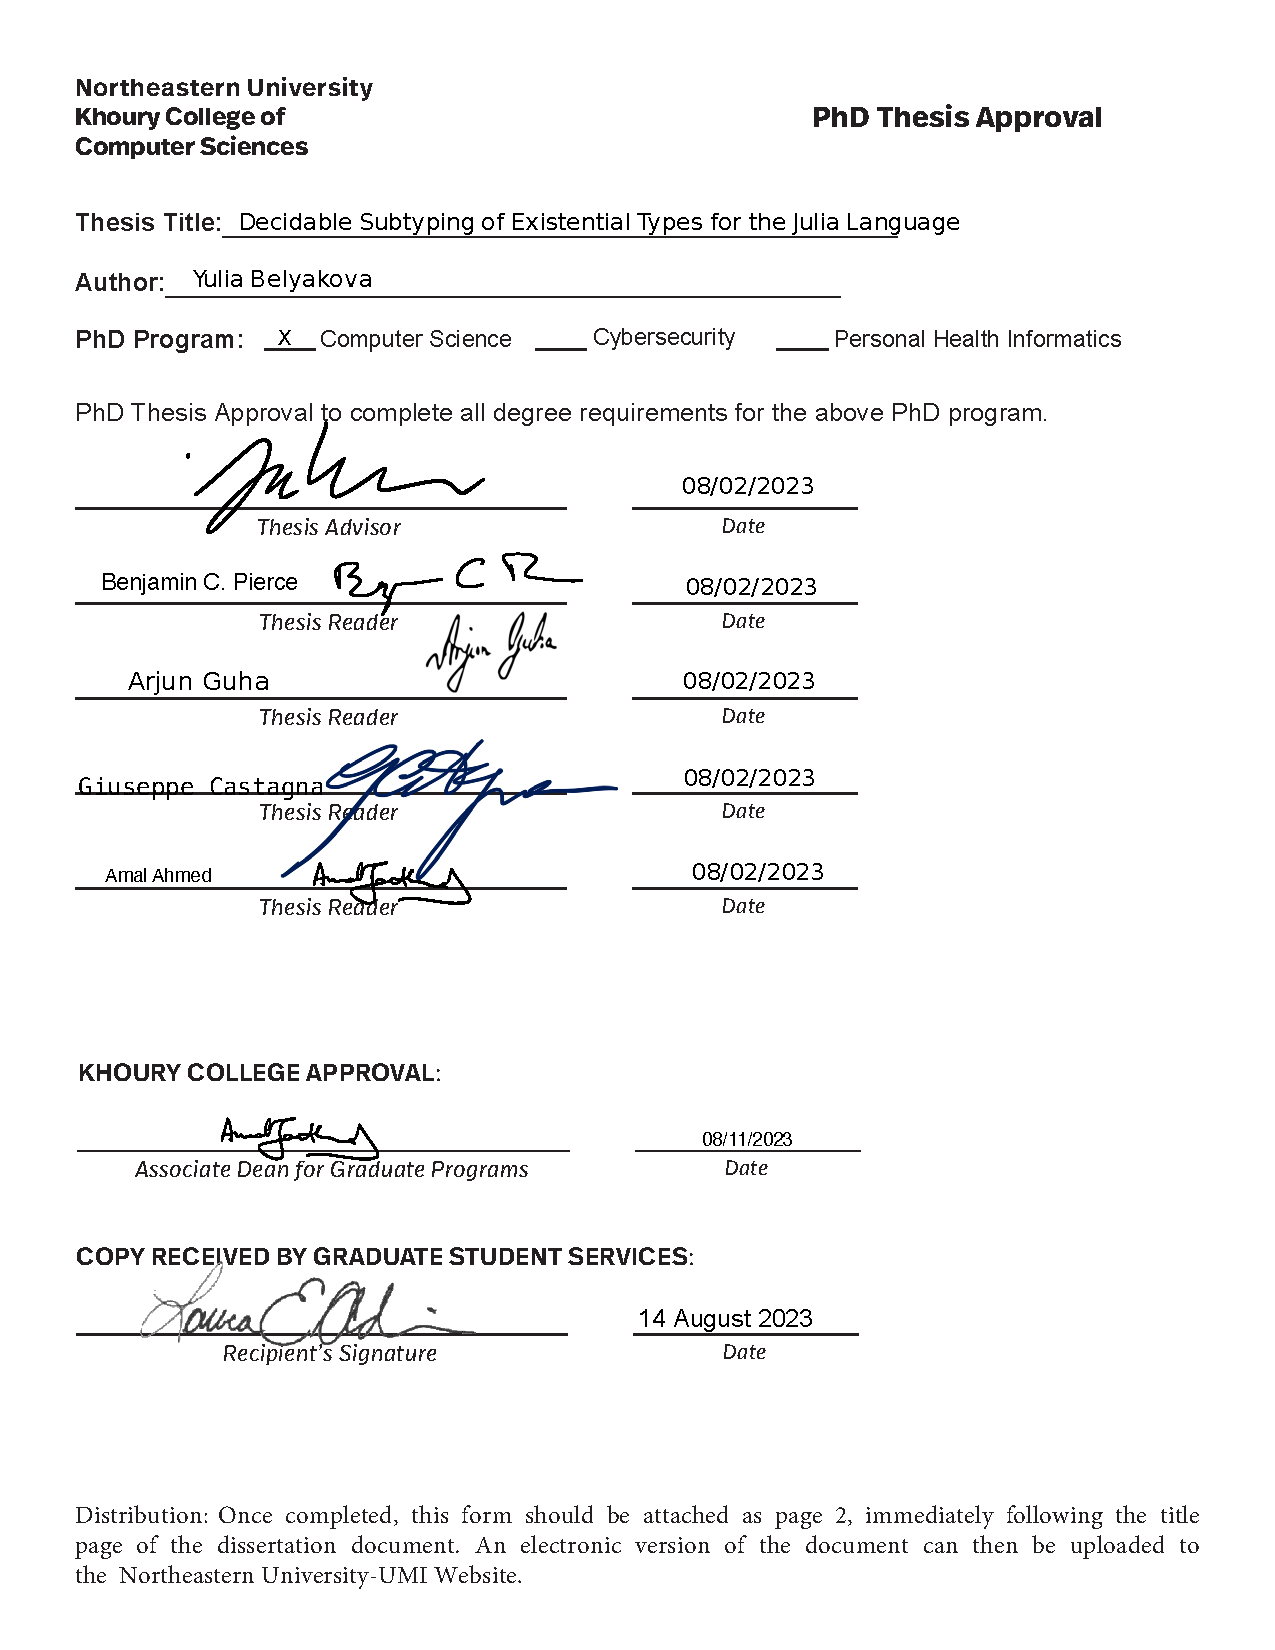
\includepdf[noautoscale]{approval.pdf}

\begin{abstract}

Julia is a dynamic, high-performance programming language
for scientific computing.
To encourage a high level of code reuse and extensibility, Julia is
designed around symmetric multiple dynamic dispatch, which allows functions
to have multiple implementations tailored to different argument types.
To resolve multiple dispatch, Julia relies on a subtype relation over a complex
language of run-time types and type annotations, 
which include set-theoretic unions, distributive tuples, parametric invariant 
types, and impredicative existential types.
Notably, subtyping in Julia is undecidable, which
manifests with a run-time stack-overflow error when program execution encounters
a subtyping query that causes the subtype checker to loop.

In this dissertation, I propose a decidable subtype relation for a restricted
language of Julia types where existential types inside invariant constructors
are limited to ones expressible with use-site variance.
To estimate migration effort that would be required for switching to the 
restricted type language, I analyze type annotations in the corpus of 9K
registered Julia packages.
Out of 2M statically identifiable type annotations in the corpus,
99.99\% satisfy the restriction, making it a viable candidate for
evolving Julia towards decidable subtyping.

\end{abstract}


%% ======================================================================
%% *********************************************************

\section{Proposal requirements}

The thesis proposal should include the relevant background materials from
literature and clearly specify the research problems to be attacked, the
techniques to be used, and a schedule of milestones towards completion.
Typically, the thesis proposal should not exceed 15 pages, excluding appendices
and bibliography.

\section{Outline}

\begin{enumerate}
  \item Introduction: overview of the problem and the proposal?
  \item Background: brief intro to Julia and an overview of types.
  \item Research problems: what is the role of types and subtyping in Julia?,
    can we define a reasonable restriction on types to achieve decidable but
    still useful subtyping relation? (With a plan to attach the problems)
  \item Related work: wildcards and existential types, decidability of bounded
    quantification, union and intersection types.
  \item Preliminary work: undesired properties of subtyping, confusion with
    diagonal types, tag-based semantic subtyping, model of Julia's JIT.
  \item Schedule of milestones.
\end{enumerate}

\chapter{Introduction}

\TODO{NOTE: this is ``the first shitty draft'', i.e. completely unedited stream
of thought.}

Julia is a dynamic, high-level language for scientific computing.
Its primary paradigm is \emph{multiple dynamic dispatch}, which allows for
high code reuse and extensibility. Although Julia does not have a static type
system, it does have an expressive language of types: both concrete user-defined
types that describe values, and abstract types that can be used in method type
annotations to specify multiple dispatch. Dispatch is implemented using
subtyping in this language of types.
The language of types is surprisingly complex, and there is no clean
specification of subtyping available to Julia users. The only reference is
effectively the implementation of subtyping, which is written in obscure C (or
C++?) code and meant to be efficient. The implementation is not very readable,
and the reason it needs to be fast is that subtyping is used at run-time.
As any function call in Julia is a dynamically dispatched call, and dispatch
relies on subtyping, it needs to be fast.

However, even the most efficient implementation of subtyping is not enough to
make the language fast. Dispatched calls can hinder optimizations. Therefore,
Julia's JIT compiler tries to remove dispatched calls and perform further
optimizations. In doing so, Julia heavily relies on type inference at run-time.
When inferred types are precise enough to ``statically'' dispatch calls, the JIT
will do so. Again, this means that subtyping is used. But furthermore, the types
are used by the type inference algorithm to guide optimizations.

As the primary purpose of types in Julia at the surface level is to describe
behaviors, the language of types is an unusual one. For example, it provides
impredicative exsitential types with bounded quantification. Furthermore,
covariant tuples and unions are distributive in Julia, which is similar to
semantic subtyping. Additionally, Julia supports a special kind of existential
types to allow for a common use case of dispatched methods: so-called diagonal
rule, where an existential variable is allowed to be instantiated only with a
concrete type. Given all this, there are concerns of understandability and
properties of the type language and subtyping in Julia.

As the first step in understanding the language of types, we tried to reverse
engineer the implementation of subtyping and provide a more readable
specification. This work is reported in \TODO{OOPSLA 18}.
While we did come up with subtyping rules that describe subtyping, we found
several issues: for example, subtyping was not transitive. There were also
several bugs in the implementation of subtyping. Furthermore, we found that the
diagonal rule works in such a way that the meaning of a type changes depending
on a subtyping relation it is checked against.
Most importantly, subtyping turns out to be undecidable in Julia. This means
that in practice, the user may face with a stack overflow at run-time because
subtyping is used for dispatching.
Another problem is that the rules we provided are hard to reason about to prove
transitivity, for example.
Thus, our first goal is to develop a specification of subtyping that is
decidable and can be reasoned about.

The way existential types are used in Julia are reminiscent of models of Java
wildcards. The key difference is that Julia's existential types are
impredicative. Interestingly, in the hope to avoid undecidability, Julia
developers intentionally restricted bounded quantification to, for example,
forbid recursive constraints on type variables.
Thus, some approaches to making subtyping decidable are not applicable, e.g.
material-shape separation \TODO{understand and explain}.

Ideally, subtyping should also be intuitive for the users. So we explore the
applicability of a semantic subtyping approach to the type language. We will
identify a property that we call tag-based semantic subtyping, and we will
strive to support this property.

Because efficiency is important for Julia, and the way it is achieved is by JIT
compilation, we explore the role of types in the JIT compiler. It turns out that
the JIT heavily relies on type inference \TODO{OOPSLA 21}. Therefore, we need to
understand what happens with types and which operations needs to be supported on
types. This will be our final guiding principle.

\chapter{Background: Julia}\label{chap:2}

\section{Overview of the Julia Language}
%% ======================================================================

Julia is a high-level, dynamic programming language for scientific computing~\cite{TODO}.
It was designed to provide good performance as well as productivity features and
the ease of use~\cite{TODO}.
For performance, Julia relies on an optimizing JIT compiler.
For productivity, the language provides garbage collection, dynamic typing, and
multiple dispatch. 

\begin{figure}[t]
%-(x::Date, y::Week) = Date(UTD(value(x) - 7*value(y)))    
\begin{julia}
-(x::BigInt) = MPZ.neg(x, y)
-(x::BigInt, y::BigInt) = MPZ.sub(x, y)
-(x::T, y::T) where T<:Union{Int16, Int32, ..., UInt128} = sub_int(x, y)
-(m::Missing, n::Number) = missing
-(A::AbstractArray{T,N} where {T,N}) = broadcast_preserving_zero_d(-, A)
\end{julia}
\caption{Several method definitions of generic function~\cjl{(-)}
in~Julia}\label{fig:code:subtraction}
\end{figure}

\tdef{Multiple dynamic dispatch}~\cite{TODO} is the core paradigm of the Julia
language. The dispatch mechanism allows a function, called \emph{generic
function}, to have multiple implementations, called \emph{methods}, that are
tailored to different argument types. For example, \figref{fig:code:subtraction}
shows several method definitions of \cjl{(-)}, which is used as both unary
negation (lines~1 and 5) and binary subtraction (lines 2--4).
At \emph{run time}\footnote{Statically typed languages often support
\emph{method overloading}. The difference between method overloading and method
dispatch is that overloading is resolved at compile time, using static types of
the arguments, whereas dispatch is resolved at run-time, using precise types
of the arguments.},
every function call in the program is dispatched to the
\emph{most specific applicable} method, which is determined based on the
types of the argument values. If such a single best method does not exist,
an error is raised.
\secref{sec:2:dispatch} describes this process in more detail, but for now,
it suffices to know that dispatch resolution relies on \tdef{subtyping}.
Notably, Julia does not allow the user to call a method of a generic function
directly: the only way to reach a method is via the dispatch mechanism.
Thus, whenever a method is called, its arguments are guaranteed to be
subtypes of the declared type annotations.
%Thus, types impact the semantics of a program despite the language being dynamically typed.

Julia has a non-trivial \tdef{language of types} \ty, some of which are
demonstrated in~\figref{fig:code:subtraction}. In addition to nominal types such
as \cjl{BigInt} and \cjl{Number}, the language also supports set-theoretic union
types (e.g. \cjl{Union\{Int16, ..., UInt128\}} in line~3),
covariant tuple types written with \cjl{Tuple} (e.g. \cjl{Tuple\{String, Number\}}),
invariant parametric types (e.g. \cjl{Vector\{T\}}),
and so-called union-all types, which are written with \cjl{where} (lines~3 and 5).
A union-all type \cjl{t where T} represents a union of types \cjl{t} for all
valid instantiations of the type variable \cjl{T}. \citet{TODO} provide a detailed
account of Julia types and their subtyping relation, and we give a brief
overview of subtyping in \secref{sec:2:subtyping}.

One of the key notions related to types in Julia is the distinction between
\emph{concrete} and \emph{abstract} types. A concrete type \gty is a type that
describes the representation of a value; for any value, its concrete type can be
obtained with the \cjl{typeof} operator. Concrete types include primitive types
such as \cjl{Int128} and composite \cjl{struct} types (either mutable or
immutable). Any concrete type definition in Julia is final: a concrete type does
not have subtypes other than itself. However, every concrete type has a single
declared supertype, which is an abstract nominal type. Such types can be used
to create a nominal subtyping hierarchy, but they cannot be instantiated with
values and have no fields. Other categories of abstract types are union types
such as \cjl{Union\{Int16,}$\ldots$\cjl{, UInt128\}}, and union-all types
such as \cjl{Vector\{T\} where T} (in Julia, such a type can be written shorter
as \cjl{Vector}). Note, however, that every particular instantiation of
\cjl{Vector}, e.g. \cjl{Vector\{Number\}}, is a concrete type.
The bottom type represented with the empty union, \cjl{Union\{\}}, is neither
concrete nor abstract: it has no values and is a subtype of all types.

\figref{fig:code:user-def-types} provides several examples of user-defined
concrete (on the left) and abstract (on the right) types. Parametric types (both
abstract and concrete) can declare lower and upper bounds on type variables;
for example, type \cjl{Rational\{T\}} requires \cjl{T} to be a subtype of
abstract \cjl{Integer}.
Supertypes in type definitions are declared to the right of~\cjl{<:}.
For example, \cjl{Int128} is a subtype of \cjl{Signed}, and \cjl{Signed} is a
subtype of \cjl{Integer}. If the supertype declaration is omitted, like in
\cjl{AbstractSet\{T\}}, the supertype defaults to \cjl{Any},
which is the supertype of all types.

It is worth noting that the language does not have a function type that would
typically be written as \cjl{T} $\rightarrow$ \cjl{S}. As mentioned above,
all function calls are dynamically dispatched to a method of the generic
function, and there is no way to directly call or
pass a particular method as an argument.
Generic functions, on the other hand, are first-class values and can be used as
method arguments, for example, \cjl{(-)} is passed to a function call in line~5
of~\figref{fig:code:subtraction}.
Every generic function~\cjl{f} has the concrete type \cjl{typeof(f)},
which is a subtype of the type of all functions \cjl{Function}.

\begin{figure}[t] 
\begin{minipage}{5.5cm}
\begin{julia}
primitive type Int128 <: Signed 128
end

struct Rational{T<:Integer} <: Real
  num::T
  den::T
end

mutable struct
  BitSet <: AbstractSet{Int}
  ...
end
\end{julia}
% struct Missing end
% bits::Vector{UInt64}
% offset::Int
\end{minipage}
\hspace{1.2cm}
\begin{minipage}{4.8cm}
\begin{julia}
abstract type Signed <: Integer
end

abstract type AbstractSet{T}
end
\end{julia}
% RefValue{T}() where {T} = new()
% RefValue{T}(x) where {T} = new(x)    
\end{minipage}
\caption{Examples of type definitions:
  concrete (left) and abstract (right)}\label{fig:code:user-def-types}
\end{figure}


\section{Multiple dispatch resolution}\label{sec:2:dispatch}
%% ======================================================================

Method resolution for a dispatched function call \cjl{f(a1, a2, ...)}
relies on subtyping between run-time argument types and method type signatures.
Argument types are combined into a tuple of concrete types
$\gty =$ \cjl{Tuple\{typeof(a1), typeof(a2), ...\}}.
Method type signature is a tuple of the declared argument types
if the method definition is not parametric, and a union-all of a tuple
if the definition is parametric.
For example, in \figref{fig:code:subtraction}, method in line~1
has the signature \cjl{Tuple\{BigInt\}}, line~4 has the signature
\cjl{Tuple\{Missing,Number\}}, and line~3 has the signature
\cjl{Tuple\{T, T\} where T <: Union\{...\}}.
Thus, for the purpose of dispatch resolution, arguments of a function call
are represented with a single concrete type \gty,
and method type signature is represented as an arbitrary type \ty.

Dispatch resolution, if successful, returns the \emph{most specific applicable
method}. Namely, for a call to generic function~\cjl{f} with the argument
type~\gty, the process can be specified as follows:
\begin{enumerate}
  \item Find all applicable methods, i.e., all method signatures \ty of the
    function~\cjl{f} such that $\gty <: \ty$ (argument type is a subtype of the
    method signature).
    If no methods are applicable, a method-not-found error is raised.
  \item Among the applicable methods $\{\ty_1, \ldots, \ty_n\}$,
    pick the method with the most specific type signature,
    i.e., $\ty_k$ such that $\forall i\in1..n, \ty_k <: \ty_i$ 
    (method type signature is a subtype of all other applicable method
    signatures). If there is no such single best method, a method-is-ambiguous
    error is raised.\footnote{Julia has extra specificity rules
    to resolve ambiguities in some cases requested by users,
    but those are not relevant to this work.}
\end{enumerate}
Julia's dispatch mechanism is \emph{symmetric}: all arguments are given
equivalent consideration as a part of subtyping of tuples.

While there are ways to optimize dispatch resolution to limit the number of
subtyping checks, the key takeaway from this section is that
in Julia, \emph{subtyping happens at run time} as a part of dynamic dispatch.
Furthermore, the following section will show that because of invariant
constructors and union-all types, even subtyping with a concrete type on the left
(i.e., $\gty <: \ty$) can require an arbitrary subtyping check $\ty_1 <: \ty_2$.

\section{Julia subtyping}\label{sec:2:subtyping}
%% ======================================================================

Subtyping in Julia largely follows the combination of
\tdef{nominal subtyping} between user-defined nominal types and
\tdef{semantic subtyping} for covariant tuple and union types.
Thus, using types from \figref{fig:code:user-def-types} as an example,
\cjl{Int128} is a subtype of \cjl{Signed}, and, transitively, of \cjl{Integer};
\cjl{BitSet} is a subtype of \cjl{AbstractSet\{Int\}} but not
\cjl{AbstractSet\{String\}}.
A~union type \cjl{Union\{t1, t2, ...\}} describes a set-theoretic union of
types \cjl{t1}, \cjl{t2}, \cjl{...}, so, for example, \cjl{Int} is a subtype of
\cjl{Union\{Signed, String\}}, and \cjl{Union\{t1, t2, ...\} <: t} if all
components \cjl{t1 <: t, t2 <: t, ...}.
Tuples in Julia are immutable, and tuple types are covariant:
\cjl{Tuple\{t1, t2, ...\}} is a subtype of \cjl{Tuple\{t1', t2'...\}} if
their corresponding components are subtypes, i.e., \cjl{t1 <: t1', t2 <: t2', ...}.
Following semantic subtyping, tuple types distribute over unions,
so types \cjl{Tuple\{Union\{Int,String\}\}} and
\cjl{Union\{Tuple\{Int\},Tuple\{String\}\}} are equivalent.

User-defined parametric types are invariant regardless of whether the type is
mutable or immutable, meaning that \cjl{Name\{t11, t12, ...\}} is a subtype of 
\cjl{Name\{t21, t22, ...\}} only if corresponding type arguments are equivalent,
i.e., \cjl{t11 <:> t21, t21 <:> t22, ...}.
Thus, while covariant \cjl{Tuple\{Int\} <: Tuple\{Signed\}},
invariant \cjl{Rational\{Int\}} is \emph{not}
a subtype of \cjl{Rational\{Signed\}}.

Abstract union-all types \cjl{t where tl<:T<:tu} are better known
in literature as \tdef{bounded existential types}, which also model
Java wildcards~\cite{TODO}\footnote{In Julia syntax, a Java wildcard type
\cjl{Foo<?>} can be written as \cjl{Foo\{T\} where T}.}.
In what follows, we will call \cjl{t where tl<:T<:tu} an existential type;
if lower (upper) bound on the type variable is omitted, it defaults to the
bottom type \cjl{Union\{\}} (top type \cjl{Any}).
Intuitively, an existential type denotes a union of \cjl{t[t'/T]} for all
instantiations of \cjl{T} such that \cjl{tl <: t' <: tu}.
Similarly to subtyping for union types,
\begin{itemize}
  \item \cjl{(t where tl<:T<:tu) <: t2} if \emph{for all} valid instantiations
    \cjl{t'} it holds that \cjl{t[t'/T] <: t2}, and
  \item \cjl{t1 <: (t where tl<:T<:tu)} if \emph{there exists} at least one 
    \cjl{t'} such that \cjl{t1 <: t[t'/T]}.
\end{itemize}
For example, \cjl{Vector\{Int\}} is a subtype of \cjl{Vector\{T\} where
T<:Integer} because \cjl{T} can be instantiated with \cjl{Int},
and \cjl{Vector\{T\} where T<:Integer} is a subtype of
\cjl{Vector\{S\} where S} because for all valid instantiations of~\cjl{T},
type variable \cjl{S} can be instantiated with the same type.
Just like with unions, tuple types distribute over existential types:
for example, types \cjl{Tuple\{Vector\{T\} where T\}}
and \cjl{Tuple\{Vector\{T\}\} where T} are equivalent.

Existential types in Julia are \emph{impredicative}:
existential quantifiers can appear anywhere in a type.
For example, type \cjl{Vector\{Matrix\{T\} where T\}} denotes a vector
of matrices with arbitrary element types.
In contrast, \cjl{Vector\{Matrix\{S\}\} where S} denotes a set vectors where
elements are matrices with the same element type.
Thus, a vector of integer matrices \cjl{Vector\{Matrix\{Int\}\}} is a subtype
of the latter, existential type, because \cjl{S} can be instantiated with
\cjl{Int}. But it is not a subtype of the former, invariant parametric type
\cjl{Vector\{Matrix\{T\} where T\}}, because type arguments \cjl{Matrix\{Int\}}
and \cjl{Matrix\{T\} where T} are not equivalent.
Note that because of the impredicativity, type arguments of invariant type
constructors such as \cjl{Vector} are arbitrarily complex. Thus, even though any
particular \cjl{Vector\{t\}} is a concrete type, its subtyping check may reduce
to subtyping of a non-concrete \cjl{t}.

Types that involve existentials, such as \cjl{Vector\{Matrix\{T\} where T\}},
are useful for representing heterogeneous data, but existential types
also represent type signatures of parametric method definitions.
It may be surprising that Julia uses existential rather than universal types,
but recall that the primary purpose of types is to serve multiple dispatch.
It is impossible to directly invoke a parametric method definition and provide
it with a type argument. Instead, the method is being dispatched to if
subtyping for the corresponding existential type succeeded. Then, in the body of
the method, the existential type is implicitly unpacked, and its witness type
is set to the instantiation induced by subtyping.
Consider the following code snippet as an example:
\begin{codeenvd}
\begin{julia}
f(v :: Vector{T}) where T = Set{T}(v)

f([5, 7, 5]) # Set{Int} with 2 elements: 5, 7
\end{julia}
\end{codeenvd}
Because \cjl{[5, 7, 5]} is a \cjl{Vector\{Int\}} and
\cjl{Tuple\{Vector\{Int\}\}} is a subtype of \cjl{Tuple\{Vector\{T\}\} where T}
as witnessed by the instantiation of \cjl{T} with \cjl{Int},
the call \cjl{f([5, 7, 5])} dispatches to the method in line~1,
and \cjl{T} in the body of the method becomes \cjl{Int}.

To support a generic programming pattern where method arguments are expected
to be of the same concrete type, Julia provides a so-called \tdef{diagonal
rule}. Consider the following method definition, which defines equality
\cjl{(==)} in terms of the built-in equality of representations \cjl{(===)}:
\begin{codeenvd}
\begin{julia}
==(x::T, y::T) where T<:Number = x === y
\end{julia}
\end{codeenvd}
If it were possible to instantiate \cjl{T} with an abstract type such as
\cjl{Integer}, the method could be called with a pair of a signed and unsigned
integer. This would be an incorrect implementation of equality, for the same bit
representation corresponds to different numbers when interpreted with and
without the sign.
To prevent such behavior, the diagonal rule states that if a type variable
appears in the type only covariantly and more than once, it can be instantiated
only with concrete types.\footnote{A similar rule applies for static resolution
of method overloading in \CSharp. An example can be found on
\href{https://fzn.fr/projects/lambdajulia/diagonalcsharp.pdf}{this page}.}
Thus, the type signature of \cjl{(==)} above,
\cjl{Tuple\{T, T\} where T<:Number} represents a restricted existential type:
it is a union of tuples \cjl{Tuple\{t, t\}} where \cjl{t} is a concrete subtype
of \cjl{Number}. The same rule applies in line~3
of~\figref{fig:code:subtraction}: built-in integer subtraction \cjl{sub_int} is
guaranteed to be called only with primitive integers of the same concrete type.

\section{Undecidability of Julia subtyping}\label{sec:2:undecidable}
%% ======================================================================

\begin{figure}
\[
\begin{array}{rcl}
  \interp{\mathit{Top}} &=& \text{\cjl{Union\{\}}}\\
  \interp{\alpha} &=& \alpha\\
  \interp{\forall\alpha\leq\ty.\ty'} &=&
    \text{\cjl{Tuple\{Ref\{}}\alpha\text{\cjl{\}, }}
    \interp{\ty'}\text{\cjl{\} where\ }}\alpha\text{\cjl{\ >:\ }}\interp{\ty}\\
\end{array}
\]
\caption{Encoding of \FSub types in Julia}\label{fig:FSub-encoding}
\end{figure}

It is not unusual for subtyping in a complex type language to be undecidable,
as happened to Java and Scala~\cite{TODO}.
In practice, for a statically-typed language, this means that the
compiler might not terminate on some programs. Although undesirable,
such undecidability, if it manifests rarely, remains an acceptable trade-off
for the sake of an expressive type system.

In a dynamically typed Julia subtyping is used at run time for dispatch
resolution. Even on rare occasions, run-time effects of
undecidability are of greater concern than the compile-time one.
Therefore, decidability of subtyping was one of the explicit goals
in the original Julia design~\cite{TODO}.
To this end, Julia disallows several features that are known to cause
undecidability: recursive constraints on type variables and
circularities in the inheritance hierarchy~\cite{TODO}.

Despite the aim of decidability, Julia subtyping is \emph{undecidable}.
As discovered by Ben Chung and Ross Tate, Julia can encode system
\FSub, which is known to be undecidable~\cite{TODO}.
\figref{fig:FSub-encoding} shows the encoding of \FSub types\footnote{Arrow
type is dropped as irrelevant to the undecidabiltiy result.},
with $\ty_1 \leq \ty_2$ of \FSub defined as
$\interp{\ty_2} <: \interp{\ty_1}$ in Julia.
Internally, Julia keeps a dedicated stack for checking subtyping
and terminates the program when the stack reaches a certain limit.
Thus, in practice, subtyping checks that showcase undecidability, such as
the Ghelli example, often manifest with a \cjl{StackOverflowError}
rather than non-termination.

\chapter{Thesis Question}\label{chap:3}

The undecidability of subtyping in Julia
can manifest itself at almost any point during the program execution,
as subtyping over a complex language of run-time types and type annotations
is an integral part of Julia's dynamic semantics.
Namely, subtyping is used to resolve function calls,
process new method definitions,
manipulate data (e.g. when adding an element to a container),
as well as during the JIT compilation.
In practice, the undecidability %of subtyping
leads to 
a run-time crash with a \cjl{StackOverflowError}.
Such an error can be particularly hard to debug,
because neither the problematic subtyping query nor its origins are available
to the user.

A number of issues related to subtyping have been reported
on the Julia bug tracker. For example,
\href{https://github.com/JuliaLang/julia/issues/41948}{\code{\#41948}}\footnote{
    \url{https://github.com/JuliaLang/julia/issues/41948}
} reports a \cjl{StackOverflowError} caused by a function definition,
which is likely linked to the undecidability;
\href{https://github.com/JuliaLang/julia/issues/33137}{\code{\#33137}}\footnote{
    \url{https://github.com/JuliaLang/julia/issues/33137}
} points out an inconsistency in subtyping; % related to the diagonal rule.
\href{https://github.com/JuliaLang/julia/issues/24166}{\code{\#24166}}\footnote{
    \url{https://github.com/JuliaLang/julia/issues/24166} 
} (now fixed) reports a problem with reflexivity and transitivity.
Overall, there are 105 open/704 closed issues labeled with ``types and
dispatch'' as of March 2023,
with 13 open/138 closed being also labeled with ``bug''
(not every issue is properly labeled as a bug,
e.g. the aforementioned
\href{https://github.com/JuliaLang/julia/issues/24166}{\code{\#24166}}).
\tabref{tab:julia-issues-stats} provides a few more data points for comparison:
for example, there are 8 open/86 closed ``codegen'' bugs
and 1 open/15 closed ``GC'' bugs.
% For context, ``bug'' and ``codegen'' are assigned to 8 open/86 closed issues
% out of 71 open/654 closed ``codegen'' issues.
% In total, ``bug'' is assigned to 226 open/2644 closed issues.
Thus, type-related concerns, including the undecidability of subtyping,
are not purely theoretical and
constitute a non-negligible portion of problems in the Julia implementation.
%Overall, there are 22 open and 114 closed issues labeled with both ``bug''
%and ``types and dispatch'' (as of December~2021). For context, ``bug'' and
%``codegen'' are assigned to 6 open and 76 closed issues, and overall, ``bug''
%is assigned to 213 open and 2477 closed issues.
%This demonstrates that type-related concerns, including undecidability of
%subtyping, are not purely theoretical: they manifest in the user code and
%constitute a non-negligible portion of problems in the Julia implementation.

\begin{table}[t]
\caption{Statistics of issues on the Julia bug tracker: open/closed (March 2023)}\label{tab:julia-issues-stats}
\vspace*{0.25em}
\centering\footnotesize
\begin{tabular}{c|ccccc}
 & types and dispatch & codegen & GC & macros & <any label> \\
\midrule
<any label> &
  92/414 & 56/246 & 24/51 & 27/36 & 3551/19238 \\
bug &
  13/138 & 8/86 & 1/15 & 5/11 & 226/2664
\end{tabular}
\end{table}

The main question addressed by my thesis research is:
\begin{quote}
\emph{Can Julia's type language be altered in a practical way
to allow for a decidable subtype relation?}
\end{quote}
Here, \emph{practical} means that most of the existing type annotations
in Julia programs would conform to the proposed type language.
The resulting relation is intended to be reflexive and transitive, as is
typical for a subtype relation. 

Furthermore, I suggest that Julia types are given a set-theoretic interpretation,
with the subtype relation matching set inclusion on the interpretations.
Although Julia was inspired by semantic subtyping, the existing subtype relation
is not consistent with the semantic approach: for example, the type 
\cjl{Tuple\{Int, Union\{\}\}} (a covariant tuple of an integer and the bottom type)
is not considered a subtype of the bottom type despite the fact that there are
no values of type \cjl{Tuple\{Int, Union\{\}\}}.

In my thesis research so far,
I have collaborated on reconstructing a specification of Julia subtyping
(OOPSLA 2018~\cite{TODO}),
defined and mechanized a set-theoretic model of a subset of Julia types
(FTfJP 2019~\cite{TODO}),
and collaborated on modeling Julia's type-specializing JIT compiler
(OOPSLA 2021~\cite{TODO}).

% The main research problem I am going to focus on is
% \tdef{decidable subtyping for the Julia language}.
% The goal is to find a decidable subtyping specification for a type language
% that is close enough to the one currently used in Julia
% and is not unreasonably restrictive.
% The latter means that the majority of types in the existing Julia packages
% are supported by the proposed specification.
% Furthermore, the type language should be suitable for the use in the rest of
% the Julia compiler.
% To tackle the problem, I will answer the following questions:
% \begin{enumerate}
%     \item \emph{How are types used in Julia and what operations on types
%       need to be supported?}
%       Clearly, types are used as type annotations in method definitions, with
%       subtyping being part of the dispatch resolution.
%       But beyond that, Julia is known to rely on type inference for optimizations
%       during JIT compilation. According to \citet{TODO}, which describes the
%       original Julia design, the type inference algorithm needs subtyping
%       but also meet, join, and widening operators.
%       As \cite{TODO} is generally outdated, the current state of Julia needs
%       to be reviewed to identify what operations on types the compiler relies on.
%     \item \emph{How complicated are types used in practice?}
%       To make subtyping decidable, I will likely need to restrict the type
%       language in some way. At the same time, the restriction should not be
%       prohibitively strong for the existing code base. Thus, an analysis of types
%       currently used in practice can provide guidance for possible restrictions.
% \end{enumerate}


\bibliography{bib/jv,bib/jl-lang,bib/all}

\end{document}
